\chapter{Projekt aplikacji}

\section{Interfejs użytkownika}\label{sec:interface_design}
Istotną częścią aplikacji są interfejsy użytkownika. Możemy tu wyróżnić wyjściowe interfejsy graficzne oraz wejściowy interfejs sterowania - klawiaturę i mysz. Diagram na rysunku \ref{fig:interface_diagram} prezentuje przejścia pomiędzy widokami prezentowanymi w sekcji \ref{sec:design_menu}.

\begin{figure}
    \centering
    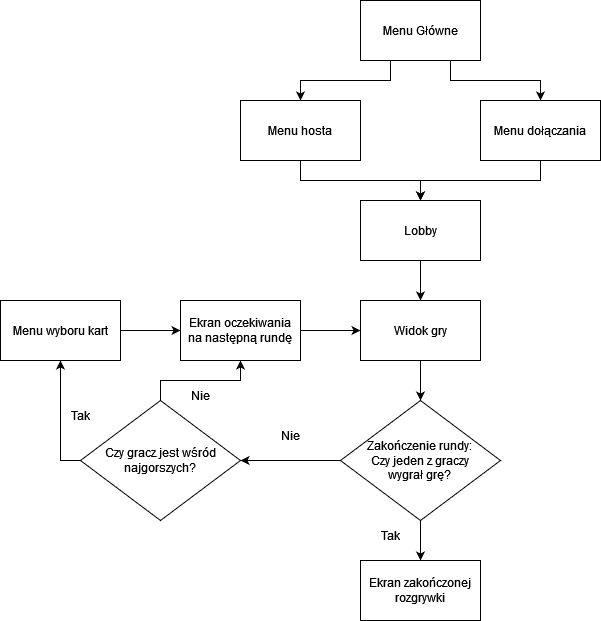
\includegraphics[width=.8\linewidth]{Images/design/DiagramMenuTanks(1).png}
    \caption{Diagram przejść między widokami.}
    \label{fig:interface_diagram}
\end{figure}

\subsection{Menu}\label{sec:design_menu}
Pierwszym ekranem widocznym dla gracza uruchamiającego grę będzie menu główne (rys. \ref{fig:main_menu}). Umożliwia ono przejście do menu hostowania gry, dołączania do gry lub wyłączenie aplikacji. 

\begin{figure}
    \centering
    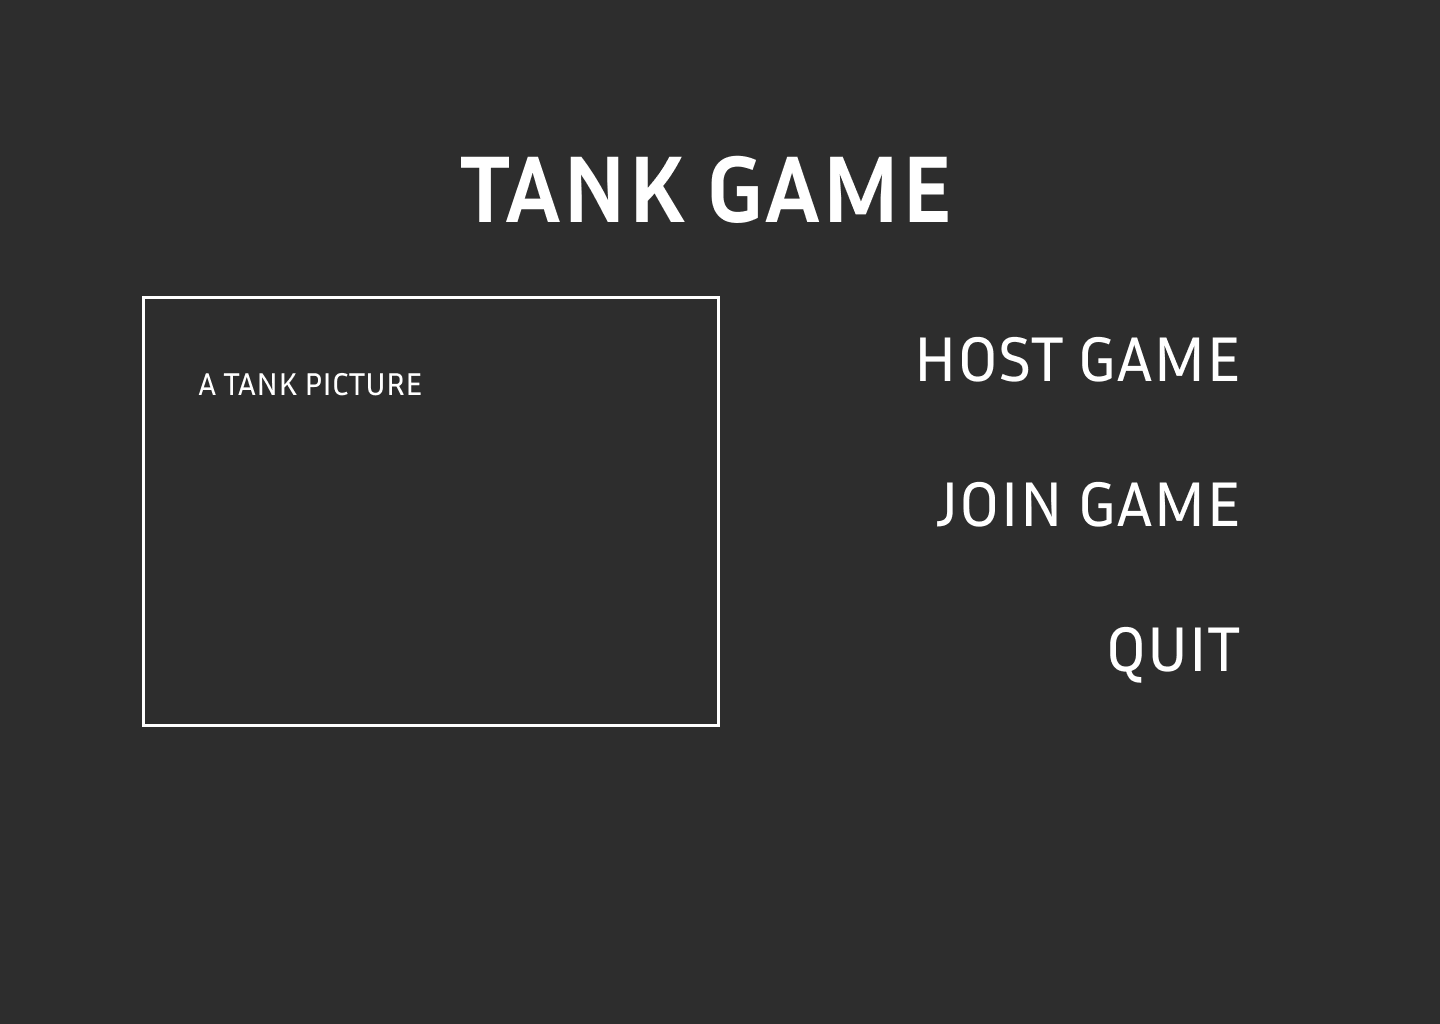
\includegraphics[width=.8\linewidth]{Images/design/Main Menu.png}
    \caption{Projekt menu głównego.}
    \label{fig:main_menu}
\end{figure}

Menu hosta (rys. \ref{fig:host_menu}) pozwala graczowi wybrać podstawowe ustawienia gry - docelową liczbę punktów zwycięstwa, oraz własne ustawienia gracza: nazwę oraz kolor. Prezentuje również adres głównego interfejsu IP. Menu dołączania (rys. \ref{fig:join_menu}) pozwala podać adres IP serwera oraz dane gracza - nazwę oraz kolor.

\begin{figure}
    \centering
    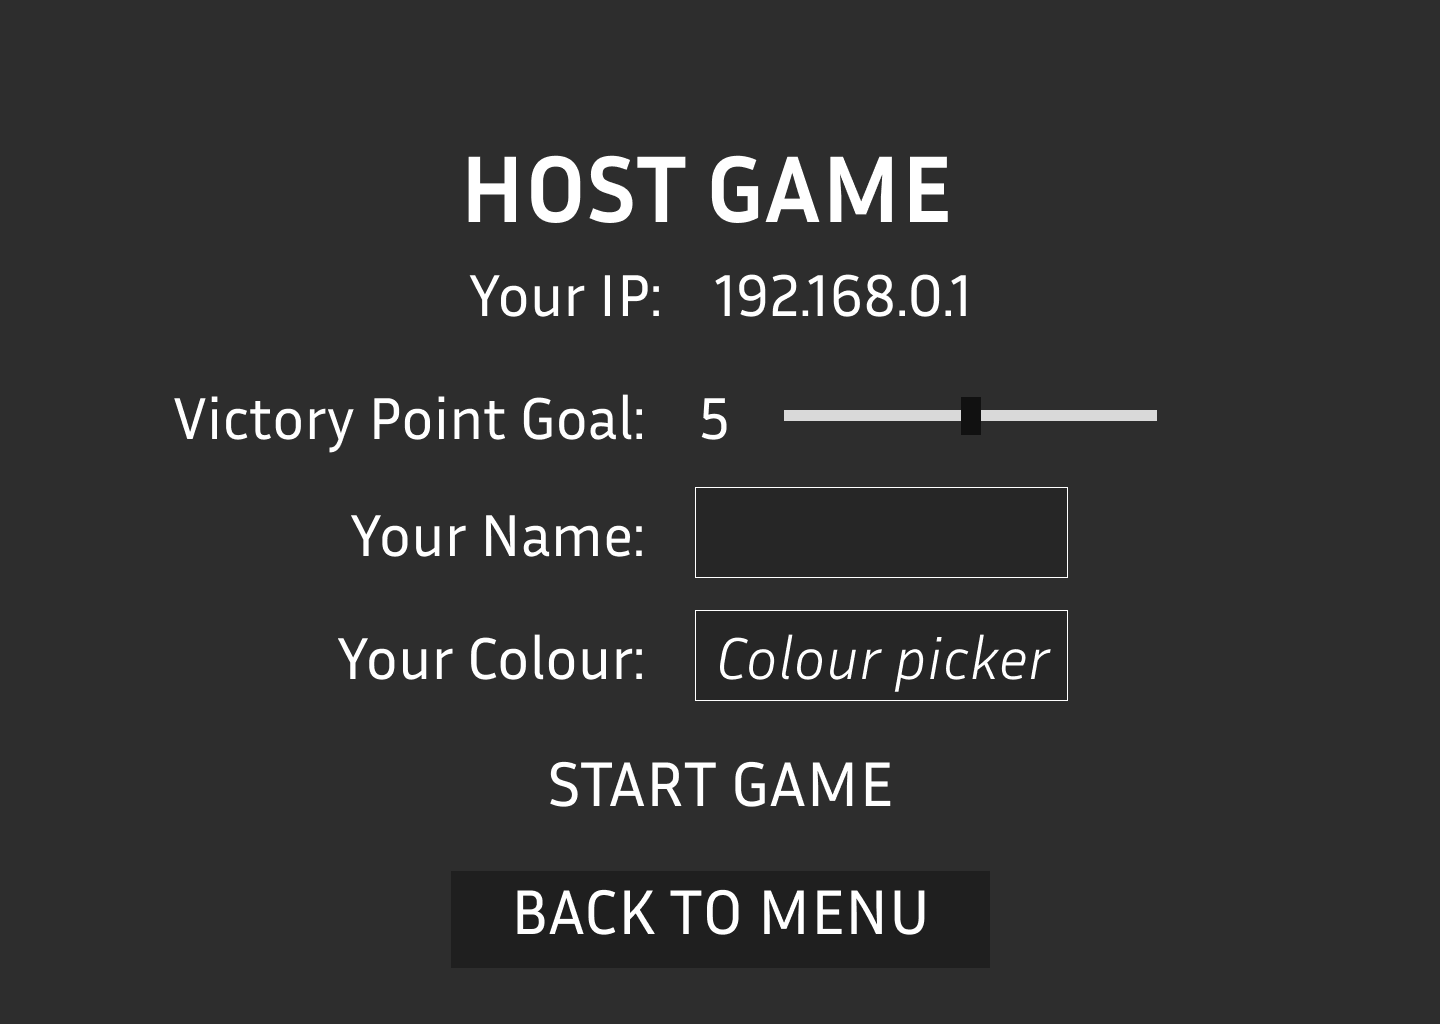
\includegraphics[width=.8\linewidth]{Images/design/Host Menu.png}
    \caption{Projekt menu hosta.}
    \label{fig:host_menu}
\end{figure}

\begin{figure}
    \centering
    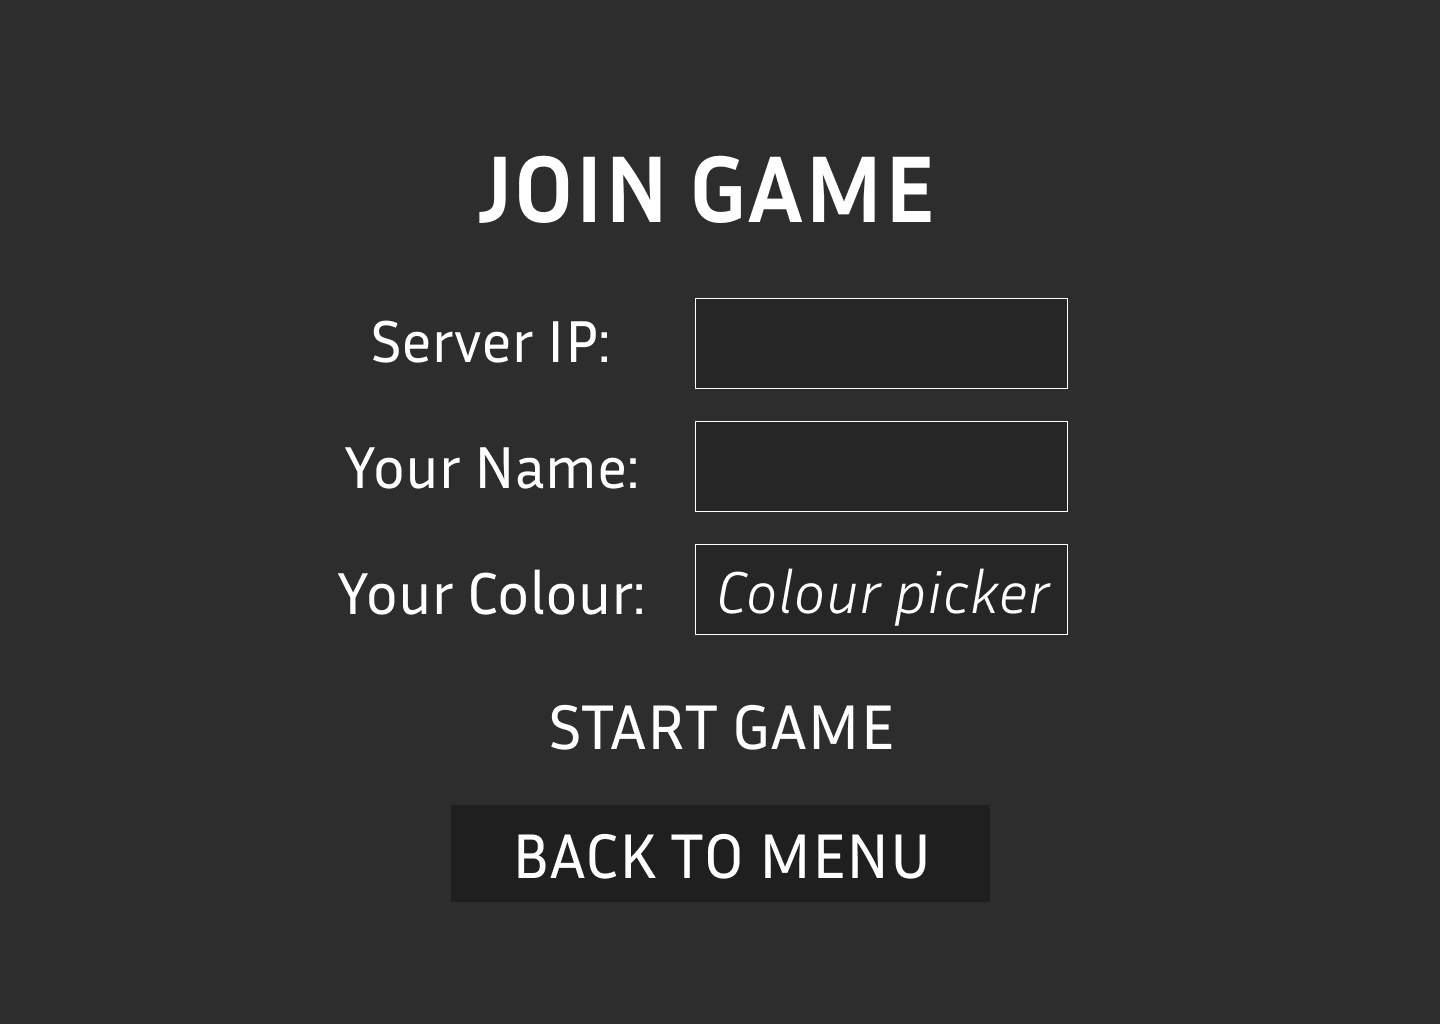
\includegraphics[width=.8\linewidth]{Images/design/Join Menu.png}
    \caption{Projekt menu dołączającego gracza.}
    \label{fig:join_menu}
\end{figure}

Po stworzeniu lub dołączeniu do serwera prezentowany jest widok poczekalni (\ref{fig:lobby_menu}). Widoczni są tu aktualnie połączeni z serwerem gracze. W tym widoku host ma możliwość rozpoczęcie gry. Gracze-klienci zamiast przycisku rozpoczynającego grę widzą jedynie komunikat o oczekiwaniu na rozpoczęcie gry przez hosta.

\begin{figure}
    \centering
    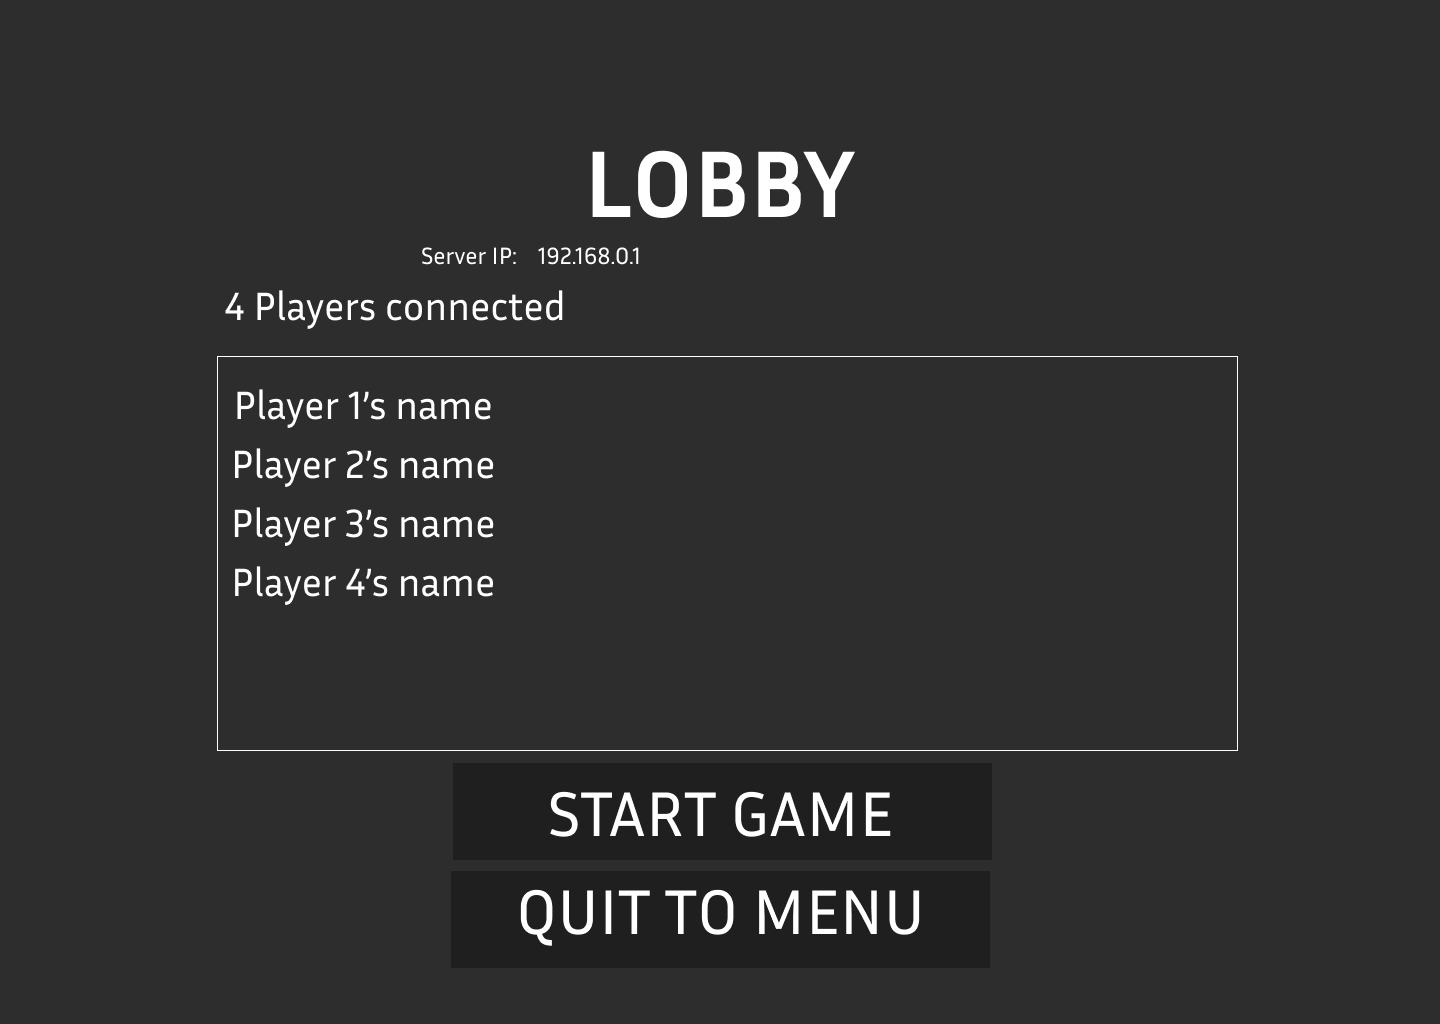
\includegraphics[width=.8\linewidth]{Images/design/Lobby Menu.png}
    \caption{Projekt menu poczekalni.}
    \label{fig:lobby_menu}
\end{figure}

Po rozpoczęciu gry przez hosta wszyscy gracze przenoszeni są do widoku gry (rys \ref{fig:game_view}). Na ekranie gracza główną część tego widoku zajmuje świat gry. W celu udostępnienia graczom niezbędnych informacji dodany został HUD\cite{beyond_hud} (ang. \emph{Heads-Up Display}, wyświetlacz przezierny). Jest to metoda wyświetlania danych tak, aby użytkownik nie musiał przenosić wzroku w miejsce inne niż jego dotychczasowy widok. W tym przypadku HUD będzie wyświetlał w prawym dolnym rogu ekranu żywotność gracza, jego maksymalną pojemność magazynku oraz aktualnie dostępną liczbę pocisków. U góry ekranu wyświetlone będą paski żywotności pozostałych graczy wraz z ich nazwami.

\begin{figure}
    \centering
    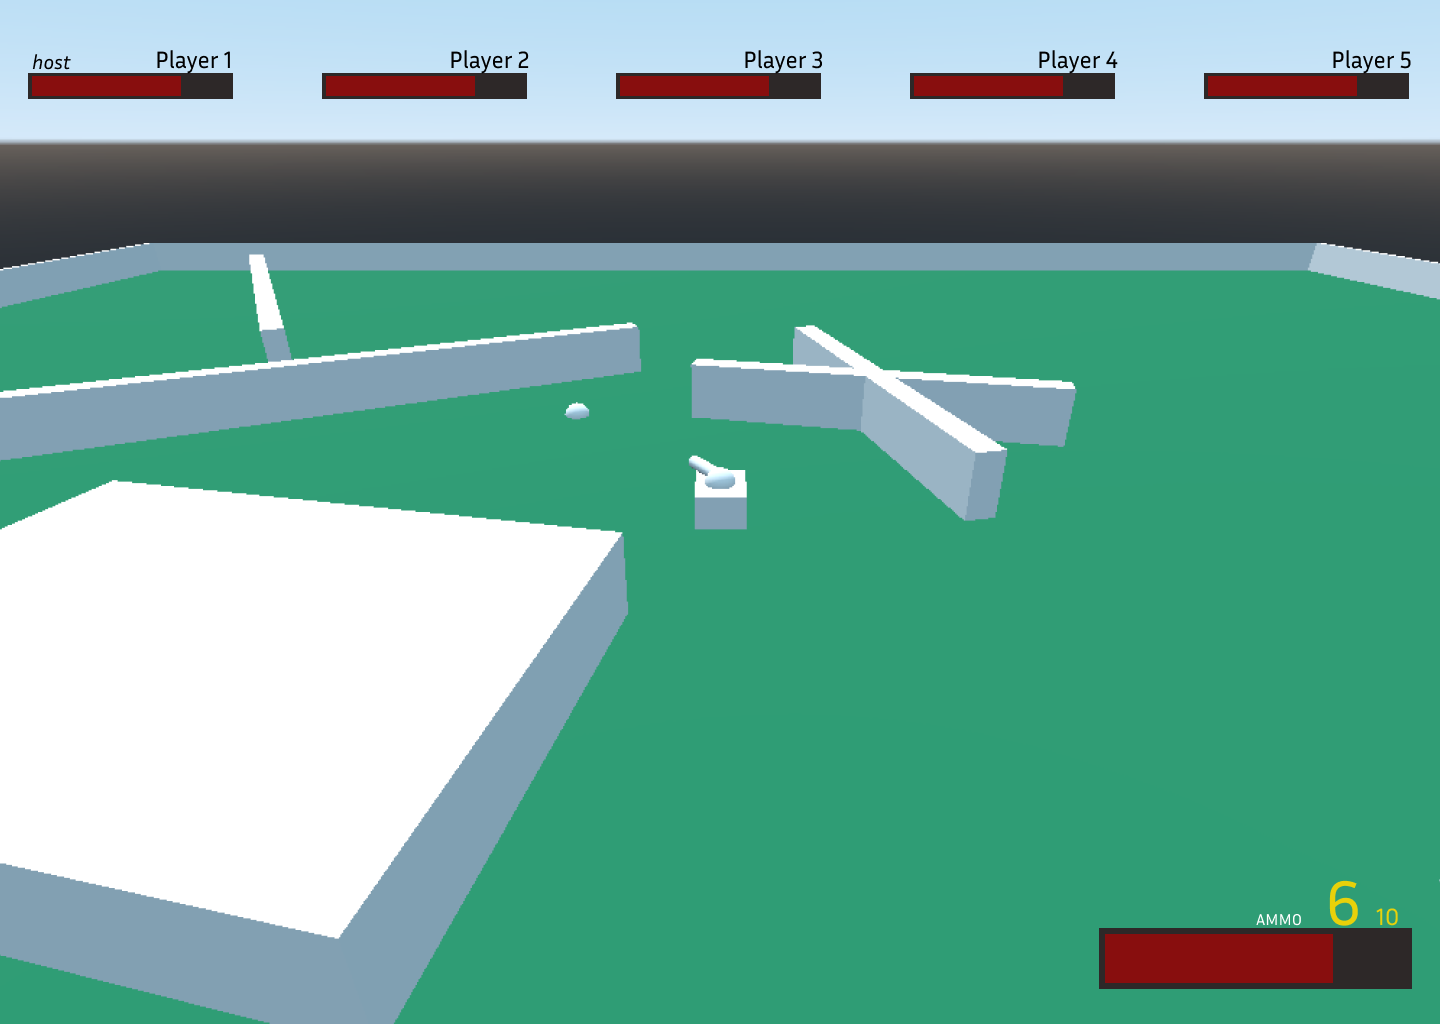
\includegraphics[width=.8\linewidth]{Images/design/Game View.png}
    \caption{Projekt interfejsu HUD.}
    \label{fig:game_view}
\end{figure}
\newpage
Między rundami graczom wyświetlane są dwa ekrany. W przypadku gdy gracz należy do najgorszych dotychczas, przenoszony jest do ekranu wyboru kart (rys. \ref{fig:cards_menu}). Prezentowane są mu tutaj trzy losowe karty - ich nazwy i opisy. Może wybrać jedną z nich a następnie potwierdzić wybór przyciskiem ,,Select''. Po wybraniu karty lub jeśli gracz nie był jednym z najgorszych prezentowany jest widok oczekiwania na pozostałych graczy (rys. \ref{fig:waiting_menu}). Widoczna jest na nim aktualna punktacja wszystkich graczy. Gdy wszyscygracze wybiorą już karty odczekiwana jest jeszcze chwila, aby ostatni z graczy mógł zapoznać się z punktacją, po czym wszyscy gracze przenoszeni są ponownie do widoku rozgrywki.

\begin{figure}
    \centering
    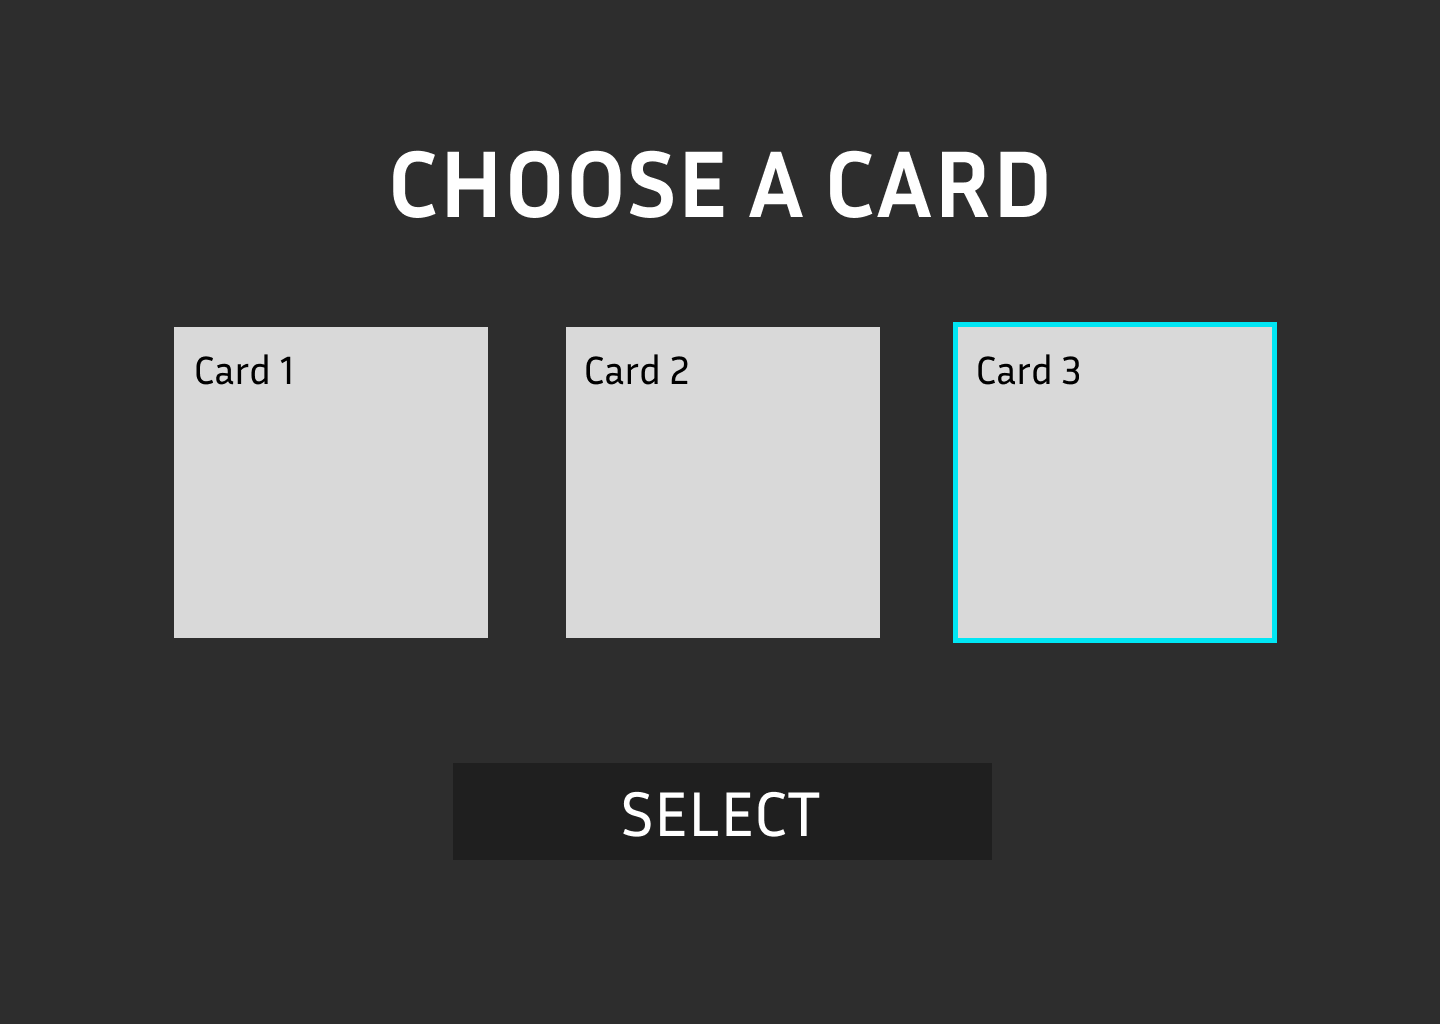
\includegraphics[width=.8\linewidth]{Images/design/Cards Menu.png}
    \caption{Projekt menu wyboru kart.}
    \label{fig:cards_menu}
\end{figure}

\begin{figure}
    \centering
    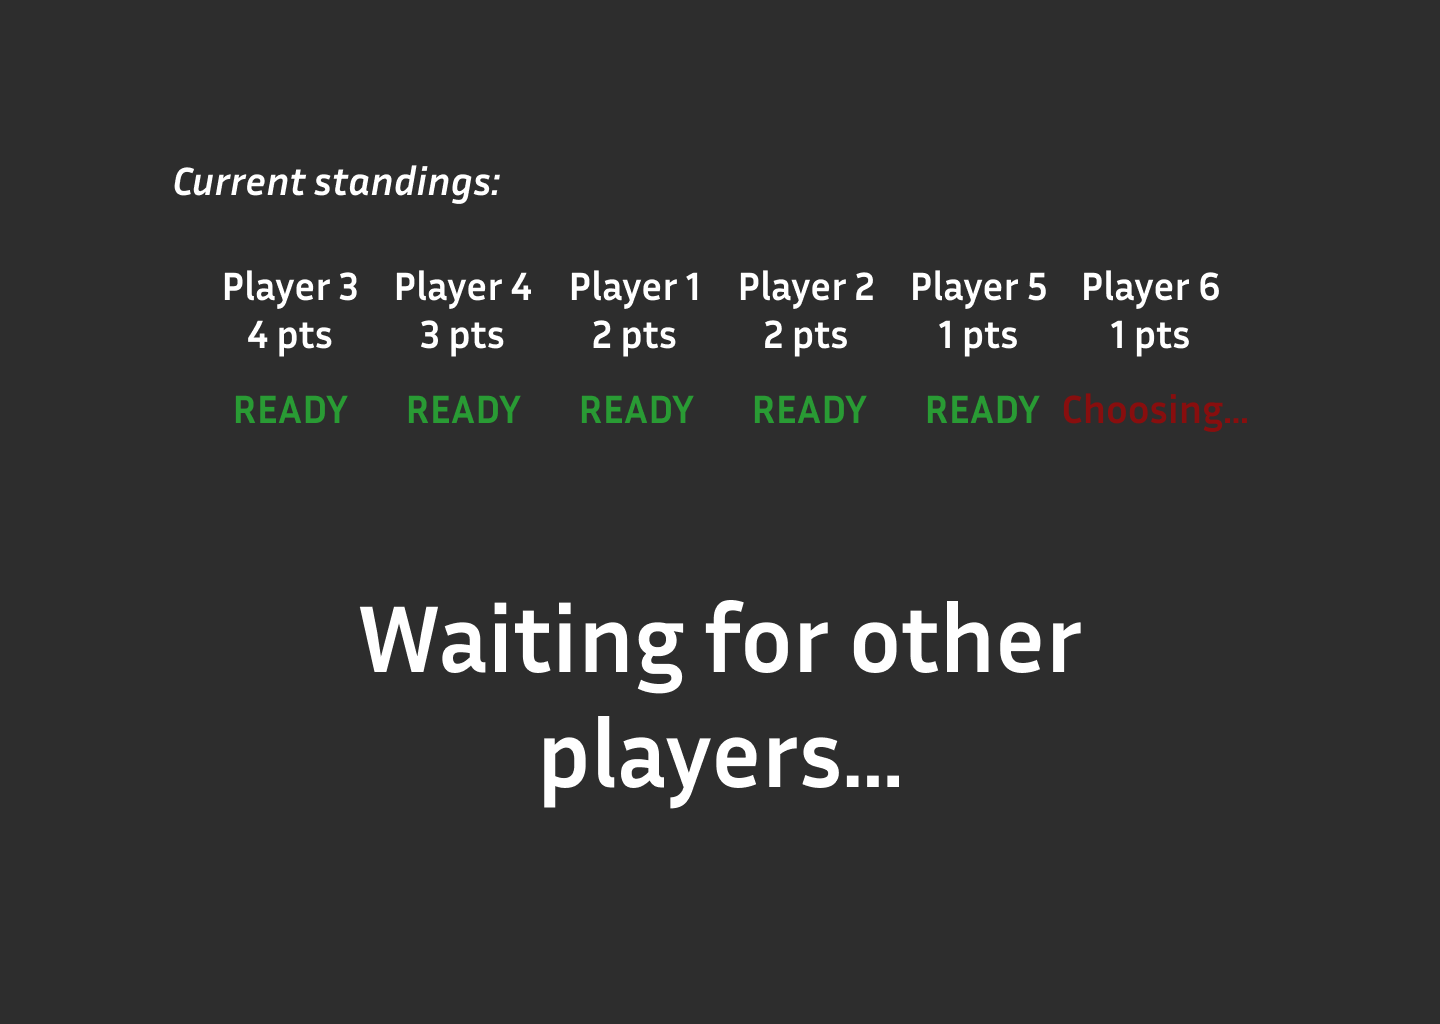
\includegraphics[width=.8\linewidth]{Images/design/Waiting Menu.png}
    \caption{Projekt menu oczekiwania między turami.}
    \label{fig:waiting_menu}
\end{figure}

W przypadku, gdy na koniec rundy jeden z graczy ma docelową liczbę punktów wszyscy gracze przenoszeni są do widoku końca rozgrywki(rys. \ref{fig:final_menu}), gdzie można zapoznać się z ostateczną punktacją.

\begin{figure}
    \centering
    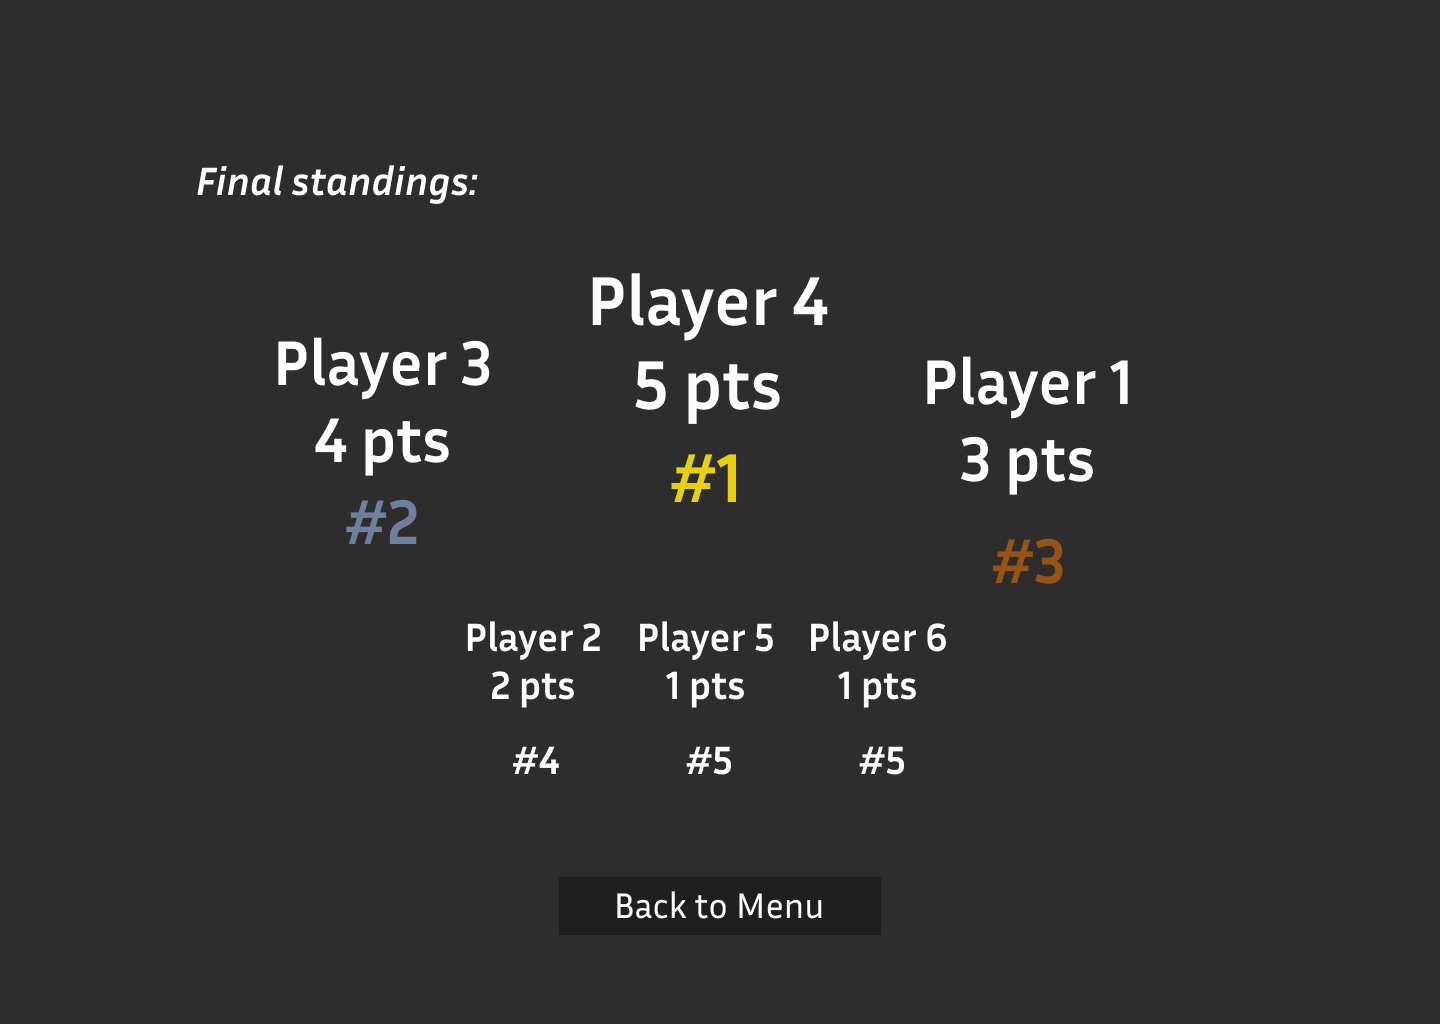
\includegraphics[width=.8\linewidth]{Images/design/Final Menu.png}
    \caption{Projekt ekranu po zakończeniu rozgrywki.}
    \label{fig:final_menu}
\end{figure}

\subsection{Schemat sterowania}

W ustawieniach projektu zostały wprowadzone akcje związane z wejściami gracza zgodne z tabelą \ref{tab:steering} i założeniami z sekcji \ref{sec:steering_concept}.

\begin{table}
    \small
    \centering
    \caption{Schemat sterowania}
    \label{tab:steering}
    \begin{tabularx}{\linewidth}{|c|c|X|}
        \hline
        Nazwa akcji & Przypisany przycisk & Opis czynności\\
        \hline \hline
        Forward & W & Poruszanie do przodu. \\
        \hline
        Back & S & Poruszanie do tyłu. \\
        \hline
        Left & A & Obrót postaci w lewo, przeciwnie do ruchu wskazówek zegara.\\
        \hline
        Right & D & Obrót postaci w prawo, zgodnie z ruchem wskazówek zegara.\\
        \hline 
        MainAction & Lewy przycisk myszy & Akcja podstawowa - strzał.\\
        \hline
    \end{tabularx}
\end{table}



\section{Projekt implementacji mechanik}
Opisane w sekcji \ref{sec:mechanics_concept} mechaniki zostaną zaimplementowane zgodnie z poniższymi projektami.

\subsection{Model danych postaci}
Atrybuty opisane w tabeli \ref{tab:stats_description} muszą być przechowywane jako pola obiektu postaci gracza. Ponadto ten obiekt przechowywać będzie dane związane z rozgrywką: nazwę gracza, jego wybrany kolor i aktualne punkty zwycięstwa. Do atrybutów postaci dodana została liczba odbić w celu ułatwienia implementacji kart.

Postać gracza przechowuje też własną prędkość jako wektor trójwymiarowy oraz prędkość kątową jako liczbę zmiennoprzecinkową. Te wartości wyrażone są jako zmiana na sekundę, w związku z tym będą musiały zostać w ten sposób wykorzystane podczas poruszania.

Wiele z atrybutów postaci reprezentuje wartości maksymalne. Analogicznie do nich wprowadzone zostaną wartości aktualne: aktualna liczba kul w magazynku i aktualne zdrowie. W celu wprowadzenia możliwości tymczasowej zmiany prędkości dla jednej z kart, do postaci dodana zostanie również aktualna maksymalna szybkość. 

Jako bufor strzału dodane zostanie pole określające liczbę klatek, przez jakie sprawdzana będzie możliwość oddania strzału. Po nieudanej próbie oddania strzału zmienna zostanie ustawiona na maksymalną wartość - 3. W każdej klatce procesu fizycznego, w której nie zostanie oddany strzał, watość bufora będzie zmniejszana o 1. Jeżeli wartość bufora była większa od 0 i oddanie strzału okaże się możliwe, strzał zostanie oddany a bufor - wyzerowany.

Ze strzałami związane są również zmienne warunkujące możliwość ich oddawania. Strzał nie jest możliwy w trzech sytuacjach: gdy postać przeładowuje broń, gdy postać właśnie oddała strzał oraz gdy gra jest zatrzymana (między rundami). Dla każdej z tych sytuacji dodane zostało oddzielne pole, określające możliwość oddania strzału.

Wartości atrybutów określające czas mają wpływ na czas oczekiwania konkretnych liczników czasu. Te liczniki zostaną dodane jako węzły do drzewa postaci oraz powiązane za pomocą sygnałów z konkretnymi metodami.

Po zmianie zdrowia oraz liczby pocisków (po strzale lub przeładowaniu) postać emituje sygnały niezbędne do aktualizowania interfejsów własnych i innych graczy.

\subsection{Poruszanie}
Wejścia gracza związane z poruszaniem będą pobierane i interpretowane w taki sam sposób jak w przygotowanym prototypie.

\subsection{Strzelanie}
Mechanika strzelania zostanie rozszerzona o buforowanie, przeładowanie oraz szybkość strzału względem prototypu. Proces strzału został przedstawiony na schemacie blokowym na rysunku \ref{fig:shoot_flowchart}.

% Ponadto ruch pocisku został zmieniony. W prototypie przemieszczanie pocisku odbywało się poprzez zmianę pozycji o odpowiedni wektor. Jest to problemem w sytuacji 


\begin{figure}
    \centering
    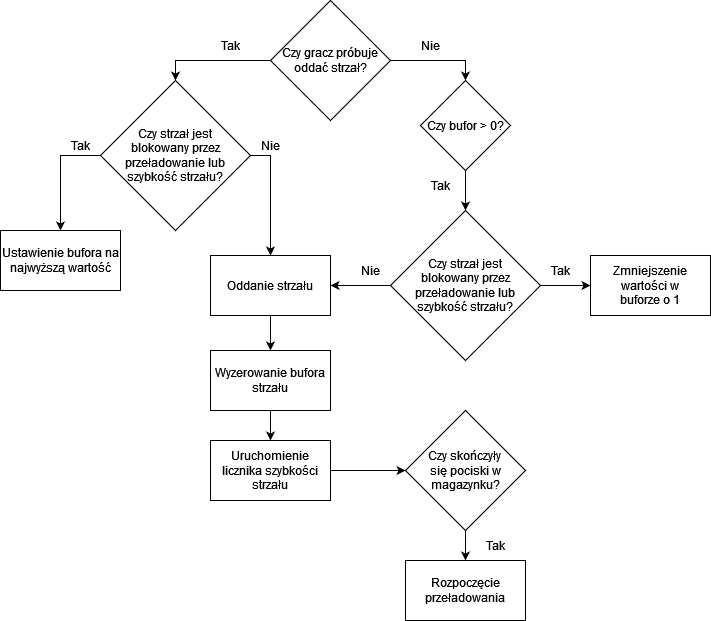
\includegraphics[width=.8\linewidth]{Images/design/ShootFlowchart(1).png}
    \caption{Schemat procesu oddawania strzału.}
    \label{fig:shoot_flowchart}
\end{figure}

\subsubsection{Wydarzenia po trafieniu}
Wydarzenia po trafieniu będą przechowywane jako obiekty implementujące wzorzec projektowy Komendy\cite{game_programming_patterns}. Taka implementacja pozwoli na potencjalne rozszerzenie wydarzeń o dodatkowe wartości lub pamięć. 

Stworzone zostaną dwa rodzaje komend - podstawowe i opóźnione. Gracz będzie przechowywał listę takich obiektów i przekazywał ją tworzonym pociskom. Po trafieniu pocisk będzie uruchamiał wszystkie komendy podstawowe, następnie ranił trafionego gracza, wykonywał odbicia, a dopiero ostatecznie, uruchamiał komendy opóźnione. Taki podział jest niezbędny dla implementacji niektórych kart.

\subsection{Zdrowie}
Postać gracza posiada określoną maksymalną żywotność oraz w każdym momencie - określoną aktualną żywotność. Po trafieniu przez pocisk zadaje on określone obrażenia, które odejmowane są od aktualnej żywotności. Trafienie rozpoczyna odliczanie licznikiem przed leczeniem. Po zakończeniu tego odliczania rozpoczyna się proces samoleczenia. Uruchamiany zostaje powtarzający się licznik leczenia. Po każdorazowym jego zakończeniu postać zostaje uleczona o konkretną wartość zależną od atrybutów postaci.

\subsection{Rundy}
Po rozpoczęciu rozgrywki przez hosta rozpoczyna się pierwsza runda. Każda z rund rozpoczyna się rozesłaniem odpowiedniego sygnału lokalnie oraz zdalnie przez hosta. Każdy z graczy ustawia wtedy odpowiednie wartości początkowe. 

Po ustawieniu tych wartości wszyscy gracze ustawiani są w odpowiednich, predefiniowanych punktach na mapie. Pozycje na mapie są ustalone jako część drzewa poziomu, ale przypisywane są graczom w losowej kolejności, dzięki czemu pozycja graczy nie będzie identyczna w każdej rundzie.

W czasie rozgrywki host zbiera i zapisuje dane na temat wyeliminowanych graczy. Gdy zostaną wyeliminowani wszyscy poza jednym, runda zostaje zakończona a host rozsyła odpowiedni sygnał lokalnie i zdalnie. 

Wraz ze zdalnym poleceniem zakończenia rundy rozsyłana jest lista najgorszych graczy oraz flaga określająca, czy gra została zakończona. Każdy z klientów oraz serwer analizuje otrzymane dane. Jeżeli flaga wskazuje na zakończenie gry, wyświetlany jest ekran końcowy. W przeciwnym wypadku, jeżeli gracz jest jednym z najgorszych wyświetlany jest ekran wyboru kart. W przeciwnym wypadku graczowi wyświetlany jest ekran oczekiwania.

Między rundami każdy z graczy wybierających karty wysyła do serwera informację o zakończeniu wyboru. Gdy każdy z graczy wybierających wyśle już taki sygnał, rozgrywka jest konynuowana w kolejnej rundzie. 

\subsection{Karty ulepszeń}\label{sec:cards_design}
Karty ulepszeń, zgodnie z koncepcją mogą zmieniać atrybuty statyczne i dodawać komendy do pocisku. Karta będzie składała się z następujących elementów:

\begin{itemize}
    \item \textbf{Nazwa} Krótka nazwa karty, reprezentująca tematycznie jej działanie.
    \item \textbf{Opis} Opis działania karty. Nie jest to szczegółowy opis a jedynie wskazanie graczowi jakie \emph{najważniejsze} cechy zmienia karta.
    \item \textbf{Zmiany atrybutów} Słownik reprezentujący zmiany atrybutów postaci. Składa się z par klucz - wartość. Kluczami są nazwy zmienianych atrybutów. Przypisaną wartością jest lista dwuelementowa w której pierwszym elementem jest sposób, w jaki zmieniana jest wartość a drugim - wartość o jaką zmieniany jest atrybut. 
    \item \textbf{Komendy po trafieniu} Lista komend dodawanych do listy komend pocisków gracza.
\end{itemize}

Zmiany atrybutów opisywane są dwoma możliwymi sposobami: mnożeniem lub dodawaniem. Oznacza to, że wartość zmiany atrybutu może zostać zastosowana jako, odpowiednio, pomnożenie aktualnej wartości przez wartość zmiany lub dodanie zmiany do aktualnej wartości. 

\section{System sieciowy}
Implementowany system sieciowy wymaga znacznej rozbudowy względem przygotowanego w ramach prototypu. Głównymi aspektami tego wprowadzanego systemu będzie synchronizacja zmian scen, w tym scena poczekalni, synchronizacja danych graczy oraz synchronizacja wydarzeń takich jak poruszanie czy trtafienia pocisków.

\subsection{Poczekalnia}
Po rozpoczęciu gry przez hosta gra uruchamiany jest poczekalni. Na tym etapie do gry przyjmowani są kolejni gracze.

Gdy do sewera podłączy się kolejny gracz sygnał o tym rozsyłany jest do wszystkich pozostałych graczy. Gracz podłączający się również otrzymuje sygnały o podłączeniu wszystkich graczy połączonych dotychczas z serwerem.

Gdy gracz dostanie informacje o połączeniu z nowym graczem przesyła temu graczowi swoje dane - nazwę oraz wybrany kolor. Te informacje są zapisywane na każdym z komputerów i prezentowane na ekranie poczekalni w liście.

Gdy wszyscy oczekiwani gracze połączą się już z serwerem host podejmuje decyzje o rozpoczęciu gry poprzez wciśnięcie odpowiedniego przycisku. Od tego momentu nie jest możliwe dołączenie kolejnych graczy. Rozpoczęcie gry nie jest możliwe, gdy żaden inny gracz nie jest połączony z serwerem.

\subsection{Przepływ danych w grze}
W czasie rozgrywki niezbędna jest synchronizacja danych pomiędzy aplikacjami. Wyróżnione zostały tu dwa rodzaje wydarzeń: interpretowane przez mistrza węzła oraz interpretowane przez serwer.

Wydarzenia interpretowane przez mistrza to takie, w których prawdziwe dane na ich temat posiada mistrz danego węzła. Rozsyła on takie dane do marionetek aby mogły one zaktualizować swoje dane. Do takich wydarzeń należą, w przypadku postaci gracza: poruszanie, strzał, synchronizacja nazwy i koloru oraz zmiana zdrowia. Z perspektywy pocisków do takich wydarzeń zaliczamy ruch i niszczenie, na przykład pod wpływem zderzenia.

Wydarzenia interpretowane przez serwer to te kluczowe dla prowadzenia rozgrywki, w związku z czym uznaje się, że to serwer jest ,,sędzią'' w ich przypadku. Ze względu na opóźnienia w komunikacji przez sieć takie wydarzenia mogą zachodzić w różnych momentach na różnych komputerach. W takich sytuacjach jedynie wydarzenia z serwera są synchronizowane. Takimi wydarzeniami są zadawanie obrażeń, eliminowanie graczy i wybór karty.